%\section{}
%\pagestyle{plain}   %Use if you do not want the fancy headers and footers... 
					 %({plain} -> just page number, {empty} -> nothing)...
					 % this will change all pages that come after this tex file...
					 % so make sure to reset the pagestyle to {fancy} at the end of this file
The methods section is partitioned into theory, which define the equations used, and the actual implementation through computational techniques. The main point of the theory is to estimate the free energy F from which the observables can be found. For example, $dF=-S\cdot dT -P\cdot dV+\mu\cdot dN$. At phase coexistence we want $\mu_{liquid}=\mu_{gas}$ and $P_{liquid}=P_{gas}$, so provided we know free energy we can simply find coexistence by setting the following:

\begin{equation}\label{eq:methodsMu}
\mu=\left(\frac{\partial F(T,V1,N)}{\partial N}\right)_{T,V1}\Bigr|_{N1}=\left(\frac{\partial F(T,V1,N)}{\partial N}\right)_{T,V1}\Bigr|_{N2}
\end{equation}

\begin{equation}\label{eq:methodsP}
P=\left(\frac{\partial F(T,V,N1)}{\partial V}\right)_{T,N1}\Bigr|_{V1}=\left(\frac{\partial F(T,V,N2)}{\partial V}\right)_{T,N2}\Bigr|_{V2}
\end{equation}

Notice that one set of derivatives are at constant V while the other set of derivatives are at constant N. Luckily this means we can simplify the derivatives by instead considering the free energy per volume; the reason this helps is both the free energy and volume are extensive quantities, which means the ratio F/V must be an intensive quantity which further means $F/V=f$ must only depend on intensive parameters. I.e. $F(T,N,V)/V=f(T,N/v)=f(T,n)$. First start simplifying eq.~\ref{eq:methodsMu} by:
\begin{equation}\label{eq:methodsMu2}
\mu=\left(\frac{\partial F(T,V,N)}{\partial N}\right)_{T,V}\cdot\frac{V}{V}=\left(\frac{\partial (F(T,V,N)/V)}{\partial (N/V)}\right)_{T,V}=\left(\frac{\partial f(T,n)}{\partial n}\right)_{T,V}
\end{equation}
At this point we know $\mu_1=\mu_2$ which combined with eq.~\ref{eq:methodsMu2} just indicates that if we plotted the free energy as a function density, then coexistence must occur when the instantaneous slope at one density matches the instantaneous slope at another density. This is useful to know, but it isn't enough to pin down a unique coexistence point. As such we must move on to simplifying eq.~\ref{eq:methodsP}:
\begin{equation}\label{eq:methodsP2}
P=\left(\frac{\partial F(T,V,N)\cdot V/V}{\partial V}\right)_{T,N}=\left(\frac{\partial f(T,n)\cdot V}{\partial V}\right)_{T,N}=f+V\cdot\left(\frac{\partial f(T,n)}{\partial V}\right)_{T,N}
\end{equation}
To simplify the last partial, use the cyclic chain rule by holding T constant throughout the process while considering the set of variables $(f,N,V)$. Proceed as follows:
$$\left(\frac{\partial X}{\partial Y}\right)_Z\cdot \left(\frac{\partial Y}{\partial Z}\right)_X\cdot
\left(\frac{\partial Z}{\partial X}\right)_Y=-1 \rightarrow$$
\begin{equation}\label{eq:P3}
\left(\frac{\partial f(T,n)}{\partial V}\right)_{N,T} \cdot\left(\frac{\partial V}{\partial N}\right)_{f(T,n),T} \cdot\left(\frac{\partial N}{\partial f(T,n)}\right)_{V,T}=-1
\end{equation}
\sloppy But we can simplify the last partial since from eq.~\ref{eq:methodsMu2} we already know that $\left(\frac{\partial N}{\partial f(T,n)}\right)_{V,T}=\frac{V}{\mu}$. Further, we can simplify the middle partial by noting $f(T,n)=constant\Rightarrow$ $f(T,N/V)=constant \Rightarrow$ $N/V=constant \Rightarrow$ $\left(\frac{\partial V}{\partial N}\right)_{f(T,n),T}=\frac{V}{N}=1/n$. Putting this all together into \ref{eq:P3} we get:
\begin{equation}\label{eq:P4}
\left(\frac{\partial f(T,n)}{\partial V}\right)_{N,T} \cdot \frac{1}{n} \cdot \frac{V}{\mu}=-1
\end{equation}
Finally we can use eq.~\ref{eq:P4} inside eq.~\ref{eq:methodsP2} to achieve the following:
\begin{equation}\label{eq:P5}
P=f+V\cdot\left( \frac{n\cdot \mu}{V} \right)=f-n\cdot\mu
\end{equation}
Having a simplified result for pressure, we can now apply the coexistence constrait that $P_1=P_2 \Rightarrow$ $f1+n1\cdot\mu=f2+n2\cdot\mu$. To compare this result with eq.~\ref{eq:methodsMu2}, solve for $\mu$ to get the following results:
\begin{equation}\label{eq:mu3p}
\mu=\frac{f2-f1}{n2-n1}
\end{equation}
\begin{equation}\label{eq:mu3}
\text{from eq.~\ref{eq:methodsMu2}: }\mu= \left(\frac{\partial f(T,n)}{\partial n}\right)_{T,V1}\Bigr|n1=\left(\frac{\partial f(T,n)}{\partial n}\right)_{T,V}\Bigr|n2
\end{equation}
The above constraints indicate that coexistence only occurs when the average slope must be equal to the instantaneous slope. This is equivalent to plotting the free energy as a function of density and finding a common tangent.

Outline:
SAFT\newline
liquid-vapor+run-absolute\newline
How comparisons were made\newline
\section{Equation Summary}
\subsection{SAFT}
\subsection{Monte Carlo Simulations}
$$Z=Z_{ideal}\cdot Z_{HS}\cdot Z_{disp}$$
$$Z_{ideal}=V^N\cdot\frac{1}{N!}\int\cdot\cdot\cdot\int e^{-\beta\cdot [P_{1}^2/{2m}+P_{2}^2/{2m}+...]}d\vec{P_1}\cdot d\vec{P_2}\cdot\cdot\cdot d\vec{P_N}$$
$$Z_{HS}=e^{-S_{exc.\infty}/k}$$
$$Z_{disp}=\frac{Z_{interaction}}{Z_{HS}}=\frac{\sum_i \alpha\cdot D(E_i)\cdot e^{-\beta\cdot E_i}}{\lim_{T\to\infty}\sum_i \alpha\cdot D(E_i)\cdot e^{-\beta\cdot E_i}}=\frac{\sum_i D(E_i)\cdot e^{-\beta\cdot E_i}}{\sum_i D(E_i)}$$
where $S_{exc.\infty}=k\cdot ln(P_{success})$ and $P_{success}$ is the probability of a successful attempt to scale an infinite box down to the size of the actual box of the simulation without hard sphere collisions; this shrinking can be done in small steps and the net sum in the change in entropy is then $S_{exc.\infty}$.

\section{Partition Function Seperation}
The partition function can be partitioned into high and low temperature regimes. At low temperatures the interactions dominate, while at high temperatures the system acts like a hard sphere system in which the entropy dominates. Both regimes can be partitioned yet again by seperating the kinetic energies into an ideal gas term. In terms of equations, we start with the partition function and seperate the summation into the three partitions:
$$\newline Z=\frac{1}{N!}\sum_i e^{-\beta\cdot E_i}
\newline Z=\frac{1}{N!}\int\cdot\cdot\cdot\int e^{-\beta\cdot [\{P_{1}^2/{2m}+P_{2}^2/{2m}+...\}+V(\vec{R_1},\vec{R_2},...)]}d\vec{P_1}\cdot d\vec{P_2}\cdot\cdot\cdot d\vec{P_N}\cdot d\vec{R_1}\cdot d\vec{R_2}\cdot\cdot\cdot d\vec{R_N}\newline$$
The momentum integrals are independent of the position integrals, so we seperate the momentum integrals which we then incorporate into an ideal gas term by multiplying by $V^N/V^N$.
$$\newline Z=\boldsymbol{Z_{ideal} \cdot \frac{1}{V^N}}\cdot \int\cdot\cdot\cdot\int e^{-\beta\cdot V(\vec{R_1},\vec{R_2},...)}d\vec{R_1}\cdot d\vec{R_2}\cdot\cdot\cdot d\vec{R_N}\newline$$
where $$Z_{ideal}=V^N\cdot\frac{1}{N!}\int\cdot\cdot\cdot\int e^{-\beta\cdot [P_{1}^2/{2m}+P_{2}^2/{2m}+...]}d\vec{P_1}\cdot d\vec{P_2}\cdot\cdot\cdot d\vec{P_N}\newline$$
After taking into account the ideal gas term, the remaining potential energy term is seperated into the low temperature and high temperature regime. At high temperatures, the atom energies are much higher than the potential well; this means the finite potential well can be considered zero. However; even at infinite temperature the atoms are assumed to be a hard sphere. This hard sphere behavior is incorporated into the partition function by multiplying by $Z_{HS}/Z_{HS}$.
$\newline Z=Z_{ideal}\cdot \boldsymbol{Z_{HS}\cdot \frac{1}{Z_{HS}}}\cdot \frac{1}{V^N}\cdot \int\cdot\cdot\cdot\int e^{-\beta\cdot V(\vec{R_1},\vec{R_2},...)}d\vec{R_1}\cdot d\vec{R_2}\cdot\cdot\cdot d\vec{R_N}\newline$
where $Z_{HS}=\frac{1}{V^N}\int\cdot\cdot\cdot\int e^{-\beta\cdot V_{HS}(\vec{R_1},\vec{R_2},...)}d\vec{R_1}\cdot d\vec{R_2}\cdot\cdot\cdot d\vec{R_N}\newline$
After taking into account the high temperature hard sphere behavior, the last part is just the ratio between the interaction and the hard sphere partition function; we call this the dispersive term.
$\newline Z=Z_{ideal}\cdot Z_{HS}\cdot \boldsymbol{\frac{Z_{interaction}}{Z_{HS}}}=Z_{ideal}\cdot Z_{HS}\cdot \boldsymbol{Z_{disp}}\newline$
where $Z_{interaction}=\frac{1}{V^N}\cdot \int\cdot\cdot\cdot\int e^{-\beta\cdot V(\vec{R_1},\vec{R_2},...)}d\vec{R_1}\cdot d\vec{R_2}\cdot\cdot\cdot d\vec{R_N}\newline$
and $Z_{disp}= \frac{Z_{interaction}}{Z_{HS}}\newline$

\subsection{Free Energy via Monte Carlo Simulations}
[FIX INTRO]
Given the separated partition function, the free energies are just the sum of the free energies due to the ideal term, the hard sphere term, and the dispersive term. The ideal term is ignored because it stays the same between theory and the Monte Carlo simulations. Due to the finite nature of the Monte Carlo simulations, the hard sphere term in the simulations aren't exactly the hard sphere terms in theory. Although we can make some corrections due to the finite nature, ultimately we have to enforce the boundary condition that at high temperature the atoms behave like hard spheres. Given this boundary condition, we are then able to define what the dispersion term should be based on estimation of the density of states.
\subsection{ideal gas free energy}
To find the ideal gas free energy we can use previous results based on knowing the entropy of the system which we can then use to find $F_{ideal}=U_{ideal}-T\cdot S_{ideal}$.
$$U_{ideal}=3/2\cdot N\cdot k\cdot T$$
$$S_{ideal^*}\approx k\cdot N \left ( ln\left [ \frac{V}{N}\left ( \frac{4\cdot \pi\cdot m}{3\cdot h^2}\cdot \frac{U}{N} \right)^{3/2} \right]+\frac{5}{2}\right )$$

The Sackur-Tetrode equation with the Stirling approximation actually does not make physical sense as the entropy per particle at constant temperature only depends on density. A simple example can show why this doesn't make sense. Consider two atoms in boxes seperated by a partition, and compare the entropy per particle to when the partition in the box has been removed. Once the partition has been removed, the two atoms can explore many more configurations than previously, which means the entropy should have increased once the two atoms were allowed to mix. Unfortunately the Sackur-Tetrode equation with Stirlings approximation would predict the entropy per particle with or without the partition should be the same. This is a bit of a problem since every box in a Monte Carlo simulation will contain exactly N particles, which means the entropy is actually lower than a real ideal gas.

The entropy problem can be fixed by using the Sackur-Tetrode equation without Stirling's approximation. Essentially use a constant density and compare the entropy per particle of a small box to the entropy per particle of a large box. The difference in entropy shows how the ideal gas entropy within a box will deviate from the expected ideal gas entropy.

$$S_{ideal}=k\cdot N \left ( ln\left [ V\cdot N!^{-1/N}\left ( \frac{4\cdot \pi\cdot m}{3\cdot h^2}\cdot\frac{U}{N} \right)^{3/2}  \right]+\frac{3}{2}\right )$$

It would be natural to think we can just incorporate this deviation in entropy for the Monte Carlo simulations, unfortunately the simulations contain an intractable problem involving the periodic nature of the simulations. The atoms in the box are repeated in a periodic way to represent the atoms in the entire fluid, however by forcing a periodic boundary condition the entire state of a fluid is now defined by only the atoms within the small box. It is very unlikely that 100 atoms can fully define a system containing an Advogadro's number of atoms, so the entropy should be much less than a realistic system. Rather than incorporate such a change in entropy, we must instead recognize that bulk properties shouldn't dependend on the boundary conditions. By applying periodic boundary conditions we are considering the small box to be the bulk. 

Although the small box does not represent the bulk, SAFT also contains the problem of using the small system to represent the bulk. Yet SAFT also enforces the boundary conditions that at high temperatures the fluid should behave like a hard sphere fluid. As such the Monte Carlo simulations are also assumed to behave like a hard sphere fluid at high temperatures, which includes both the ideal term and the hard sphere term.

\subsection{hard sphere free energy}
The hard sphere partition function can be found by calculating the excess entropy at $T\to\infty$. This can be seen as follows:
$$Z_{exc}=Z_{HS}\cdot Z_{disp}\Rightarrow$$
$$\newline F_{exc}=-k\cdot T\cdot ln(Z_{exc})=-k\cdot T\cdot ln(Z_{HS})-k\cdot T\cdot ln(Z_{disp})\Rightarrow $$
$$\newline S_{exc.\infty}=\lim_{T\to\infty}-\left ( \frac{\partial F_{exc}}{\partial T} \right ) _{V,N} \text{ but }\lim_{T\to\infty}Z_{exc}=\text{constant}\Rightarrow$$
$$\newline S_{exc.\infty}=-k\cdot ln(Z_{HS.\infty})-k\cdot ln(Z_{disp.\infty})$$
$$\newline \text{but }Z_{HS}\text{ is constant and }Z_{disp.\infty}=Z_{interaction.\infty}/Z_{HS}=Z_{HS}/Z_{HS}=1 \Rightarrow$$
$$S_{exc.\infty}=-k\cdot ln(Z_{HS})-k\cdot ln(1)=-k\cdot ln(Z_{HS}) \Rightarrow$$
$$\newline Z_{HS}=e^{-S_{exc.\infty}/k}$$

To find the hard sphere partition function, we need to find the maximum excess entropy as $T\to\infty$. The method used to find the maximum excess entroy starts by considering N atoms in an extremely large box at a very large temperature. The atoms in the large box should behave like an ideal gas, so the entropy of this large box is a known starting point. Then all atom positions are scaled relative to a corner as the origin. Although each individual atom can now exist within a smaller box, it is not guaranteed an atom will not overlap with another atom after the positions are scaled down.

What we can observe is the probability that a particular scaling fails, and from this probability the change in entropy from the bigger box down to the smaller box can be calculated. The details are as follows:
$$\newline F=U-T\cdot S \Rightarrow  S=(U-F)/T\approx -F/T=k\cdot ln(Z)$$
$$\text{let }Z_{small}=\text{partition function of the smaller box}\newline$$
$$\text{let }Z_{big}=\text{partition function of the bigger box}\newline$$
$$\Delta S=S_{small}-S_{big}=k\cdot ln(Z_{small})-k\cdot ln(Z_{big})=k\cdot ln(Z_{small}/Z_{big})\newline$$
From here note that although every configuration in the bigger box is not guaranteed to scale down into the smaller box, it is guaranteed that the smaller box can be expanded into the bigger box. This means there is a mapping from the partition function in the smaller box to the bigger box; as such we can break $Z_{big}$ into valid and invalid configurations where the valid configurations are guaranteed to shrink down into the smaller box and the invalid configurations are not. The $\Delta S$ can then be simplified by making a connection between $Z_{small}$ and $Z_{valid}$.
$$\newline \text{let }Z_{big}=Z_{valid}+Z_{invalid}\newline$$
$$\text{but }Z_{small}\text{ maps into }Z_{valid} \Rightarrow Z_{small}=\alpha\cdot z_{valid}\text{ for some constant } \alpha\newline$$
This constant $\alpha$ can be found directly by looking at the partition function of both the big and small box. All configurations in the small box can be mapped into the valid regions of the large box which means to find $\alpha$ all we have to do is rewrite $Z_{small}$ in terms of $Z_{big}$.
$$\newline Z_{small}=\frac{1}{N!}\int\cdot\cdot\cdot\int e^{-\beta\cdot [\{P_{1}^2/{2m}+P_{2}^2/{2m}+...\}+V(\vec{R_1},\vec{R_2},...)]}d\vec{P_1}\cdot d\vec{P_2}\cdot\cdot\cdot d\vec{P_N}\cdot d\vec{R_1}\cdot d\vec{R_2}\cdot\cdot\cdot d\vec{R_N}$$
The momentum integrals are assumed independent of the spatial integrals, so we can leave them out of the comparison.
$$\newline Z_{small}\propto\frac{1}{N!}\int\cdot\cdot\cdot\int e^{-\beta\cdot [V(\vec{R_1},\vec{R_2},...)]} d\vec{R_1}\cdot d\vec{R_2}\cdot\cdot\cdot d\vec{R_N}$$
From here make the change of variables for each spatial coordinate to remap the integral from the small partition funciton into the big partition function, and in the process the scaling term $\alpha$ is found.
$$\newline Z_{small}\propto\frac{1}{N!}\int\cdot\cdot\cdot\int e^{-\beta\cdot [V(\vec{R_1},\vec{R_2},...)]} d\vec{R_1}\cdot \left(\frac{L_{big}}{L_{small}}\right)^3 \cdot d\vec{R_2}\cdot \left(\frac{L_{big}}{L_{small}}\right)^3 \cdot\cdot\cdot d\vec{R_N}\cdot \left(\frac{L_{big}}{L_{small}}\right)^3 \cdot \boldsymbol{\left(\frac{L_{small}}{L_{big}}\right)^{3N}}$$
$$\newline Z_{small}=\left(\frac{L_{small}}{L_{big}}\right)^{3N}\cdot Z_{big}=\left(\frac{V_{small}}{V_{big}}\right)^N\cdot Z_{big}\doteq\alpha\cdot Z_{big} \Rightarrow$$
$$\alpha=(V_{small}/V_{big})^N$$
Now that $\alpha$ is known, we can get back to finding the entropy.
$$\Delta S=k\cdot ln(Z_{small}/Z_{big})=k\cdot ln(\alpha\cdot Z_{valid}/Z_{big})\newline$$
$$\Delta S=k\cdot ln(\frac{V_{small}^N}{V_{big}^N}\cdot Z_{valid}/Z_{big})\newline$$
$$\text{but }Z_{valid}/Z_{big}=\text{probability of success when scaling}=P_{success}\Rightarrow\newline$$
$$\Delta S=k\cdot ln(\frac{V_{small}^N}{V_{big}^N}\cdot P_{success}
)\newline$$
At this point this $\Delta S$ represents the total change in entropy from squeezing the box. However; only the change in excess free entropy was wanted. To compensate, simpy subrtract the change in entropy due to the ideal gas using constant temperature and constant number of atoms.
$$\Delta S_{exc.\infty}=\Delta S_{\infty}-\Delta S_{ideal.\infty}$$
$$\text{but }\Delta S_{ideal.\infty}=k\cdot N\cdot ln(V_{small}/V_{big})\Rightarrow$$
$$\Delta S_{exc.\infty}=k\cdot ln(\frac{V_{small}^N}{V_{big}^N}\cdot P_{success})-k\cdot N\cdot ln(V_{small}/V_{big})$$
$$\Delta S_{exc.\infty}=k\cdot ln(P_{success})$$


\subsection{dispersive free energy}
The dispersive term is found by estimating the density of states using a * method. The main problem is the density of states is found by sampling the energy levels, but the relative distribution of energy levels is not unique to a single density of states. In other words, the partition function can be changed by an arbitrary factor without actually changing the total energy. This can be seen as follows:

Suppose $$Z=\sum_i D(E_i)\cdot e^{-\beta\cdot E_i}$$

then $$U=\sum_i E_i\cdot D(E_i)\cdot e^{-\beta\cdot E_i}/Z\newline$$

Now suppose we let $$D_2(E_i)=\alpha\cdot D(E_i)$$

then $$Z_2=\sum_i \alpha\cdot D(E_i)\cdot e^{-\beta\cdot E_i}=\alpha\cdot Z\Rightarrow\newline$$
$$U_2=\sum_i E_i\cdot D_2(E_i)\cdot e^{-\beta\cdot E_i}/Z_2$$
$$\newline U_2=\sum_i E_i\cdot \boldsymbol{\alpha}\cdot D(E_i)\cdot e^{-\beta\cdot E_i}/(\boldsymbol{\alpha}\cdot Z)$$
$$\newline U_2=\sum_i E_i\cdot D(E_i)\cdot e^{-\beta\cdot E_i}/Z$$
$$\newline U_2=U\newline$$
Basically the partition function will define the total energy at all temperatures, but knowing the total energy at all temperatures will not define a unique partition function. Specifically, the partition function up to some arbitrary factor will give the same total energy. This is a bit problematic considering the method to find the density of states makes observations of the total energy to estimate the density of states, which then results in a density of states that is only defined up to some unknown factor.

To get around this problem of an unknown factor in the density of states, note that the dispersive partition function will go towards one as T approaches infinity. This happens because $Z_{disp}$ is the ratio of the interaction term to the hard sphere term, and the interaction term approaches the hard sphere term as the temperature increases. Essentially we can leave the unkown $\alpha$ term alone, and it will show up in both the interaction and hard sphere partition function.

That is: $$Z_{disp}=\frac{Z_{interaction}}{Z_{HS}}=\frac{\sum_i \alpha\cdot D(E_i)\cdot e^{-beta\cdot E_i}}{\lim_{T\to\infty}\sum_i \alpha\cdot D(E_i)\cdot e^{-\beta\cdot E_i}}=\frac{\sum_i D(E_i)\cdot e^{-\beta\cdot E_i}}{\sum_i D(E_i)}$$
%\pagebreak
\newpage
\section{Computation}
\begin{figure}[h]
\vspace*{-7mm}
\hspace*{-6mm}
	\centering
	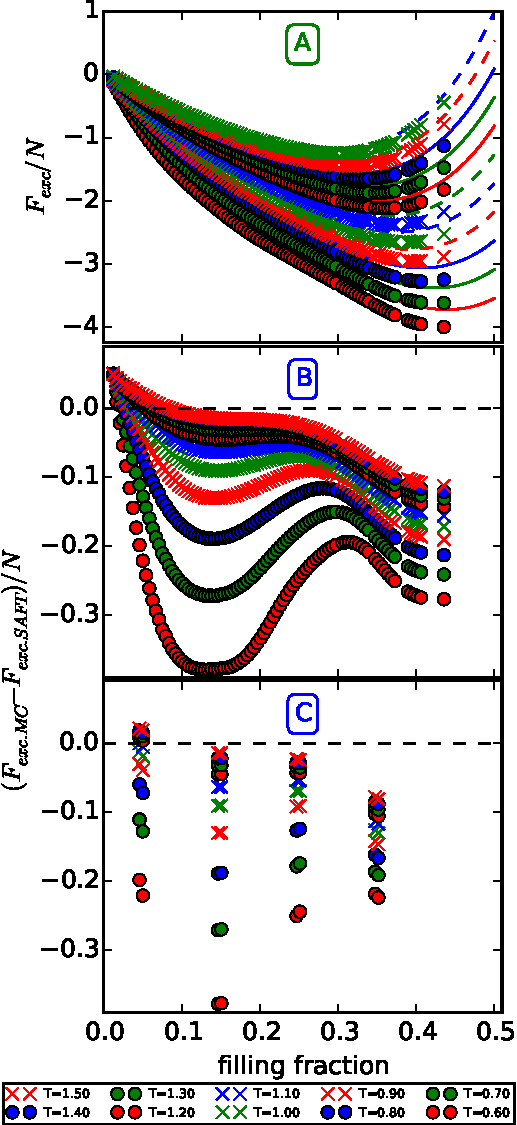
\includegraphics[scale=.9]{FdispVsff-scrunched-ww1.50-L10.00-i0.pdf}
	\caption{Caption for this image.}
	\label{fig:FdispVsff}
\end{figure}

\begin{figure}[h]
\vspace*{-7mm}
\hspace*{-6mm}
	\centering
	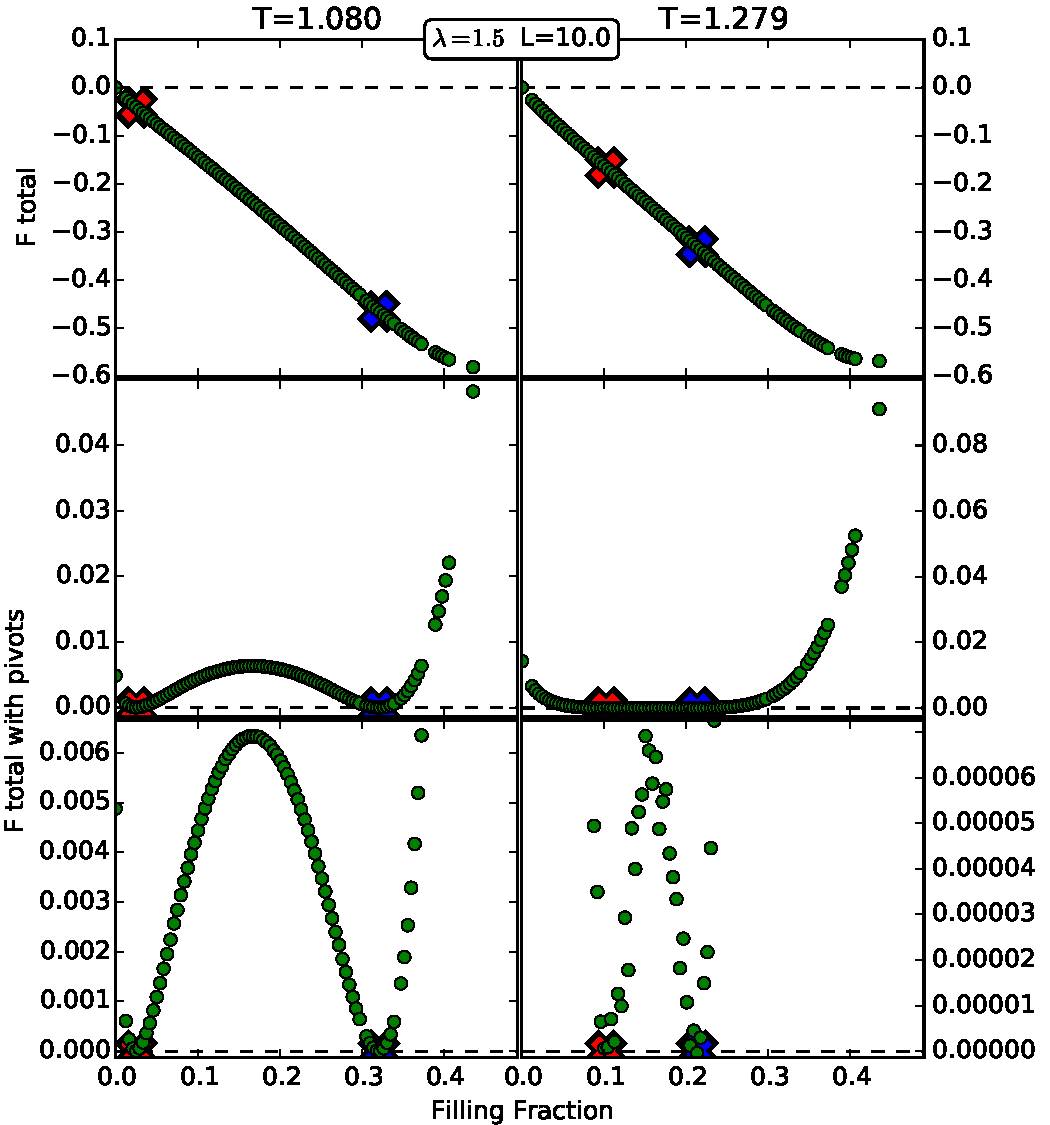
\includegraphics[scale=.9]{commonTangent.pdf}
	\caption{\scriptsize Here the common tangent method is demonstrated. The free energy at a particular temperature is plotted as a funciton of density. The two points highlighted by red and blue X's on the curve share a common tangent; this means both points will have the same pressure and chemical potential. The left and right set of plots shows how the signal to noise ratio changes as the temperature increases. Far from the critical point the signal is relatively strong, while the near the critical point the noise becomes significant. To prevent the loss of the signal, first start at a low temperature where the signal is strong. Then gradually increase the temperature while finding common tangents. As the temperature and noise increases, the previous solutions at a slightly lower temperature can be used as a guess for the new higher temperature.}
	\label{fig:FdispVsff}
\end{figure}



%\pagestyle{fancy}   % Reset all pages after this file to fnacy headers